\chapter{\label{results}Results}



\section{Relative error}

Figure \ref{fig:rel-error-100000} shows the absolute value of the relative error ($|\varepsilon_{rel}|$) for 100 000 highscore updates. After 100 000 highscore updates the dynamic bucket-tables' relative error remains practically constant at $0.05 \%$. For the static bucket-table, the error grows from $7 \%$ to $0.25 \%$.

\begin{figure}[h!]
  \centering
  \caption{Development of the relative error for 100 000 highscore updates.}
  \label{fig:rel-error-100000}
  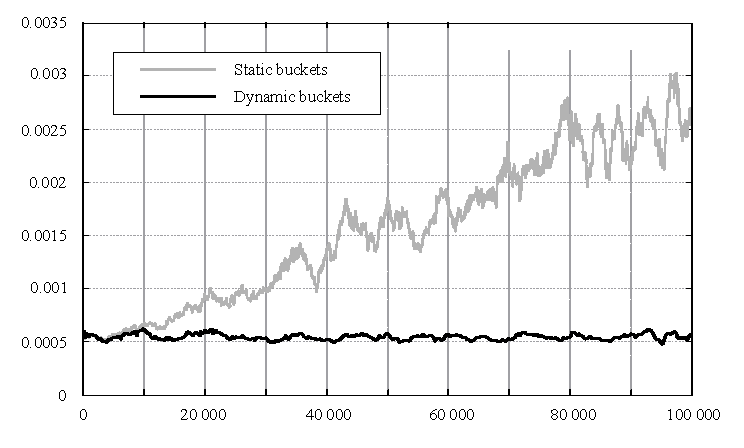
\includegraphics[width=13cm]{img/rel-error-100000.eps}
\end{figure}

Figure \ref{fig:rel-error-10000} is a plot of the same relative error but for approximations 1 -- 10 000. It shows where the difference between the two algorithms starts to be significant. At $t_1$, the relative error for the original algorithm is at its maximum in the range 1 -- 4000, also slightly higher for the algorithm with dynamic buckets. Also, the relative error is practically the same after 4 000 updates. At $t_2$ the relative error exceeds the largest relative error with the original algorithm\footnote{The results would not be exactly the same if the experiment had been run a number of times with different random seeds to create an average relative error. This is also the reason for causing ambiguity by not specifying $t_1$ and $t_2$ exactly.}.


\begin{table}[h]
  \vspace{4mm}
  \begin{center}
    \begin{tabular}{ r | c c c c c }
      Approx n ($\times 1000$) & {[}1-20)           & {[}20-40) & {[}40-60) & {[}60-80) & {[}80-100)    \\ \hline
                Mean               & 0.07    & 0.11     & 0.16     & 0.21     & 0.25   \\
                Median             & 0.03    & 0.04     & 0.05     & 0.06     & 0.08   \\
                Standard Deviation & 0.19    & 0.43     & 0.64     & 0.86     & 0.96   \\
                Maximum            & 6.34    & 20.5     & 21.9     & 28.4     & 33.7   \\

    \end{tabular} 
    \caption{Relative error with static buckets, \%}
    \label{table:results-a}
  \end{center} 
\end{table}

\begin{table}[h]
  \vspace{4mm}
  \begin{center}
    \begin{tabular}{ r | c c c c c }
      Approx n ($\times 1000$) & {[}1-20)           & {[}20-40) & {[}40-60) & {[}60-80) & {[}80-100)    \\ \hline               
                Mean               & 0.06    & 0.05    & 0.05    & 0.05     & 0.05 \\
                Median             & 0.03    & 0.03    & 0.03    & 0.03     & 0.02 \\
                Standard Deviation & 0.14    & 0.11    & 0.12    & 0.12     & 0.13 \\
                Maximum            & 6.76    & 2.50    & 4.40    & 4.21     & 5.83 \\
    \end{tabular} 
    \caption{Relative error with dynamic buckets}
    \label{table:results-b}
  \end{center} 
\end{table}

\begin{figure}[h!]
  \centering
  \caption{Relative error for 10 000 highscore updates.}
  \label{fig:rel-error-10000}
  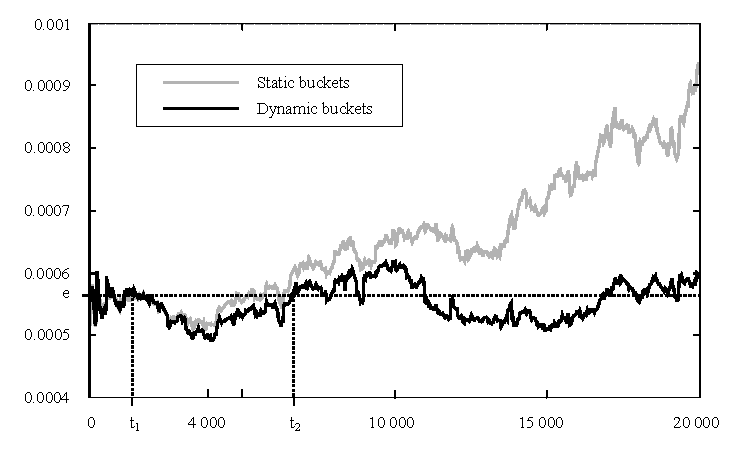
\includegraphics[width=13cm]{img/rel-error-10000.eps}
\end{figure}

\section{Execution time}

The execution time is measured on a local development server and not on the cloud platform targeted. The local development server is an Intel Core i7-6700K with 16 GB of RAM which at the time of writing has the fastest single-thread performance available. The virtual machines (instances) provided by Google App Engine are far less powerful. For example, the least powerful instance have CPU-limit corresponding to 600 MHz on an unspecified architecture and 128 MB of RAM\footnote{\hhref{https://cloud.google.com/appengine/docs/about-the-standard-environment\#instance\_classes}}. No measurements have been done to determine what kind of scaling factor would apply when translating the results to a production environment.

\subsection*{Cost of making one approximation}
The cost for approximating one rank is composed of a share of the cost for building a bucket-table and the cost for making the approximation. With the dynamic bucket-table approach, adjusting and storing the bucket-table adds an additional cost to each approximation. The cost for making an approximation for the two methods compared are presented in Table \ref{table:exec-time}. Both runs of the experiment had about one hundred outliers ($>100$ ms) which affect the mean significantly by  $0.6$ ms in both cases.

\begin{table}[h]
  \vspace{4mm}
  \begin{center}
    \begin{tabular}{ r | c c c }
Time (ms) & Static buckets     & Dynamic buckets & Difference \\ \hline
Mean               & 5.914           & 7.604  & 1.690 \\
Median             & 5               & 7      & 2 \\
Standard Deviation & 17.418          & 19.029 & 1.611 \\
Maximum            & 702             & 757   & 55
    \end{tabular} 
    \caption{CPU-time in milliseconds (ms)}
    \label{table:exec-time}
  \end{center} 
\end{table}

\subsection*{Cost of creating a bucket-table}

Building a bucket-table for 100 000 highscores takes 10 205 ms in average. The time does not vary much between test runs (Table \ref{table:bucket-table-creation}).

\begin{table}[h]
  \vspace{4mm}
  \begin{center}
    \begin{tabular}{ r | c }
      & Bucket-table creation time (ms) \\ \hline               
                Mean               & 10 205  \\
                Median             & 10 341  \\
                Standard Deviation & 140.98  \\
                Maximum            & 10 520  \\
    \end{tabular} 
    \caption{Bucket-table creation time, 100 000 highscores. Sample size: 5.}
    \label{table:bucket-table-creation}
  \end{center} 
\end{table}
